\hfill\break
\justifying
\textbf{DTW 1-NN}
	\hfill\break
	\justifying
	Un modelo obligatorio como punto de partirda entre las bastas alternativas de técnicas que atienden el problema TSC, es a través de una combinación del algoritmo DTW y el modelo \textit{k-NN}, para la clasificación de sequencias dependientes del tiempo, mostrando sus capacidades de precisión y robustez cuando comparado con técnicas más poderosas[21].
	
	\hfill\break
	\justifying
	Esta robusta técnica combina la medida de similitud entre secuencias de tiempo DTW y el algoritmo de clasificación k-NN(\textit{k Nearest Neighbours}) en su variante con \textit{k=1}, parámetro definido de forma empírica por inifindad de trabajos anteriores y para conformar actualmente el método base en el problema de TSC por la creciente aceptación por parte de la comunidad.
	
	\hfill\break
	\justifying
	En esta variante del algoritmo k-NN, se sustituye la distancia Euclideana como función de medida entre los datos, por la medida de similitud DTW entre series de tiempo, resultando en su gran capacidad de clasificación con una buena precisión. Aún con los beneficios que otorga el modelo referencia, es importante revisar los detrimentos de la técnica frente a las limitaciones y condicionantes naturales de la problemática que se atiende. La gran debilidad de este algoritmo reside en la complejidad y tiempo de cálculo, dado principalmente por el uso de función de medida a DTW en el modelo clasificador.
	
	\hfill\break
	\justifying
	La complejidad cuadrática de DTW, $O(N^2)$, cuando se evalua la similitud de la series de tiempo que se intenta predecir con respecto al número de instancias que conforman el conjunto de datos de ''entrenamiento'', incrementa significativamente el número de cálculos derivado de la conformación de la matriz de costo del algoritmo. Frente a esta situación, se ha buscado la optimización del algoritmo utilizando las restricciones, en un intento de disminuir la complejidad en la conformación de la matriz de costo acumulada, inevitablemente requiriendo el aprendizaje del tamaño óptimo del parametro \textit{w}, restringiendo los cálculos a elementos más cercanos a la diagonal.
	
	\hfill\break
	\justifying
	La versión desarrollda experimentalmente en este trabajo, implementa la técnica de optimización del tamaño de la ventana DTW[17], en la búsqueda de satisfacer las condiciones de la solución que exígen un modelo optimizado sin dejar de lado una buena precisión en la predicción.
	
\hfill\break
\justifying
\textbf{Modelo SAX-DTW}
	\hfill\break
	\justifying
	Técnica propuesta en el paper \textit{''Gesture recognition using Symbolic Aggregate Approximation and Dynamic Time Warping on motion data''}[13], como el método mas preciso de entre los 3 evaluados, y que supera a los demás al reportar una razón promedio de clasificación correcta igual al 99.21\%.
	
	\hfill\break
	\justifying
	El método se basa en la coexistencia del algoritmo SAX y la función de medida DTW, logrando combinar las mejores características de ambos métodos; La efectividad y baja complejidad de SAX, con la insensibilidad de DTW a las fluctuaciones de velocidad durante la ejecución de un gesto[13].
	
	\hfill\break
	\justifying
	Este segundo método, al igual que el de referencia, utiliza como clasificador subyacente a 1-NN, pero implementado como función de distancia, la propia distancia SAX modificada para implementar la alineación óptima de DTW.
	
	\hfill\break
	\justifying
	La totalidad de las secuencias temporales serán discretizadas a la representación SAX, tanto las instancias de conjunto de ''entrenamiento'', como los nuevos patrones ingresados para su etiquetado mediante predicción.
	
	\hfill\break
	\justifying
	Importante para el método SAX aclarar los valores de los parámetros utilizados. En el \textit{paper} desarrollan sus experimentos con un valor para el número de palabras igual a 32(Representación PAA), y un tamaño de alfabeto igual a 7.
	
	\hfill\break
	\justifying
	Finalmente la funcion de medida adopta el concepto de la distancia entre 2 símbolos SAX, con un modificación que ocupa el camino óptimo de deformación, proponiendo una comparación de la distancia entre símbolos relacionados por el camino DTW en vez de la comparación por defecto entre los pares de símbolos, y que elige al par que corresponde al símbolo de cada una de las cadenas en el mismo índice(una comparación de distancia Euclideana en el ámbito discreto simbólico de SAX). En la Figura 8 se ilustra el uso del método SAX-DTW.
	
	\hfill\break
	\justifying
	La implementación del algoritmo DTW en este método exige la optimización del parámetro \textit{w}, como restricción en forma de banda Sakoe-Chiba, aplicándose también durante los resultados de la experimentación, el método de aprendizaje del tamaño óptimo de ventana[17].
	
	\begin{minipage}{\linewidth}
		\centering
		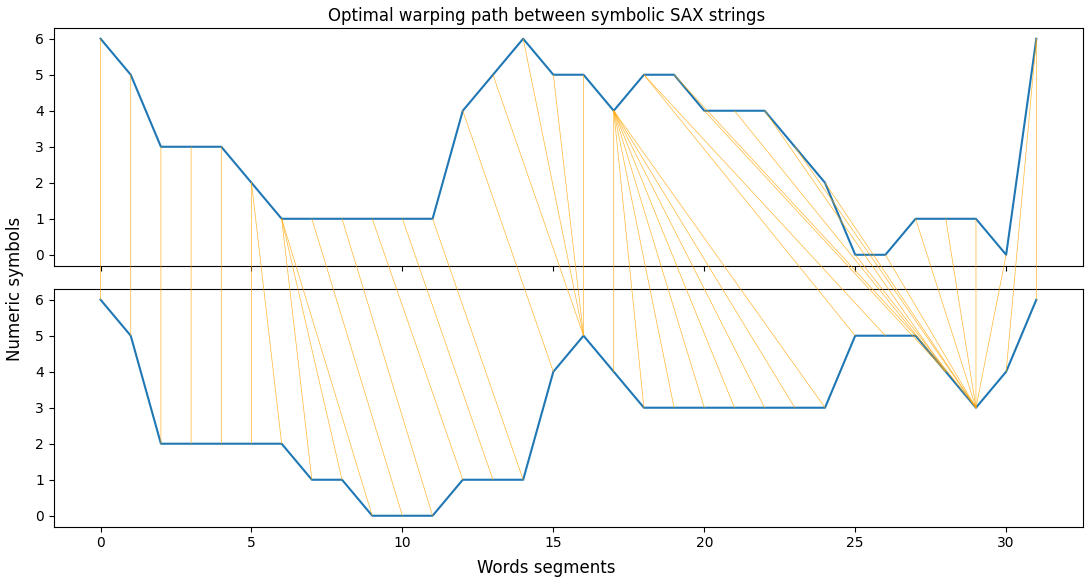
\includegraphics[width=\linewidth]{Imagenes/SAX_DTW.png}
		\captionof{figure}{Algoritmo del camino de deformación óptima calculada por DTW sobre 2 cadenas simbólicas SAX.}
	\end{minipage}
	
\hfill\break
\justifying
\textbf{Método vectores de atributos distancia DTW de series de tiempo SAX}
	\hfill\break
	\justifying
	Como método original propuesto en este trabajo, se busca al igual que el segundo método, la coexistencia y adición de los beneficios que ofrece la disminución dimensional y discretización por parte de las representaciones SAX, con la robustez en el proceso de medición de la similitud de DTW para series con extensión y velocidades distintas. Aún cuando ambos algoritmos se implementan en un mismo modelo, el enfoque y filosofía de funcionamiento del modelo difiere del segundo, implementado una técnica desarrollada en el \textit{paper}[22] y que propone representar a una serie de tiempo en conformando los atributos de distancias DTW en comparación de cada ejemplo de entrenamiento[22].
	
	\hfill\break
	\justifying
	Así como el método toma inspiración de las técnicas desarrolladas en ambos artículos[17,22], ninguna de las técnicas se aplica fielmente tal y como los describen los autores en sus respectivos trabajos.
	
	\hfill\break
	\justifying
	Un cambio especialmente importante en comparación a los métodos descritos anteriormente, es la implementación de un algoritmo \textit{Machine Learning} mucho más robusto al sencillo k-NN. ocupándose un clasificador de soporte vectorial, y que forma parte de las ventajas y posibilidades de mejora al conformarse vectores de atributos distancia DTW[22].
	
	\hfill\break
	\justifying
	Apalancándose del hecho de que la manera más sencilla de obtener una mejora en la precisión de la clasificación para secuencias dependientes del tiempo, es la implementación de un método basado en características(Representación estadística o simbólica definida para una serie de tiempo), se requiere la transformación de los datos en un espacio alternativo donde las características discriminatorias pueden ser más facilmente detectables que un clasificador más complejos en el tiempo[6]. 
	
	\hfill\break
	\justifying
	El manejo de la totalidad de series de tiempo se realiza mediante las cadenas simbólicas resultantes del algoritmo SAX, que proveé además de una transformación a un espacio alternativo de dominio simbólico, una reducción dimensional, lo que traduce en una simplificación de la complejidad. Esto implica que ninguna de las etapas siguientes pueda realizarse sin antes transformar las secuencias en cadenas simbólicas con número de palabras iguales a 64 y su discretización en el dominio de valores con un alfabeto tamaño 9.
	
	\hfill\break
	\justifying
	Pensando en aprovechar todo el potencial de las similitudes calculadas por DTW, se escoge un alfabeto numérico en las representaciones SAX, con la finalidad de utilizar sin realizar una previa modificación de los símbolos la distancia DTW. Este alfabeto numérico de tamaño 9, ofrece los dígitos enteros dentro el rango $[0,8]$ como el conjunto de símbolos que conformand las cadenas SAX.
	
	\hfill\break
	\textbf{Proceso de entrenamiento}
	\justifying
	Cuando se involucra un método de \textit{Machine Learning} como SVC, el modelo debe pasar por una etapa de entrenamiento antes de poder ofrecer la tarea de predicción, situación que no sucede con el algoritmo k-NN de los métodos previos, pues realmente la etapa de entrenamiento y predicción sucede en un proceso integral.
	
	\hfill\break
	\justifying
	La creación de los vectores de atributos en este método es escencial, no solo por la posibilidad que ofrece de aplicarse como entrada a modelos robustos de \textit{Machine Learning}, pero por que además diverge del paper[22] en el que se inspira, y se toma una interpretación alternativa que impacta positivamente las etapa de entrenamiento y predicción, pero siendo de mayor relavancia su ventaja durante la predicción; Disminuyendo significativamente el tiempo de cálculo y complejidad requerido para la creación del vector de instancias por cada secuencia temporal.
	
	\hfill\break
	\justifying
	Tomando un enfoque alternativo a la creación del vector de atributos, antes de pasar si quiera a esta etapa, se requiere crear una cadena simbólica representante de cada clase existente en el conjunto de datos, y como requsito se exige la estratificación del conjunto para mantener la equiprobabilidad de las clases durante el entrenamiento.
	
	\hfill\break
	\justifying
	La fabricación del conjunto de cadenas representantes se logra mediante el promediado de
	todos los vectores existentes en el conjunto de datos que pertenecen a una misma clase, y el método más efectivo para lograr un representante fidedigno de cada etiqueta es DBA[20].
	
	\hfill\break
	\justifying
	Este conjunto de representantes resultante se convierte a partir de su cálculo, en el conjunto de cadenas simbólicas más importantes del modelo. El hecho de que mediante la similitud DTW de estos representantes con los vectores destinados al entrenamiento y posteriormente los nuevos patrones a ser predecidos, exige la preservación del conjunto durante la vida útil del modelo entrenado. A pesar de tratarse de un algoritmo determinístico que sugiere el recálculo del conjunto de representantes frente a la pérdida de este, si la elección de la serie de tiempo abreviada inicial \textit{A} se obtiene por un proceso aleatorio, el cálculo una segunda vez del conjunto de representantes significaría desechar el modelo entrenado para volver a crear las instancias de entrenamiento con este nuevo conjunto.
	
	\hfill\break
	\justifying
	Creado el conjunto de cadenas representantes de cada clase, se calculan los vectores de atributos distancia DTW entre la instancia de entrenamiento y los representantes de clase(es importante el orden en que se ingresan ambas cadenas simbólicas, pues la operación de similitud DTW no es conmutativa), ingresándolos en el modelo SCV para iniciar la etapa de entrenamiento.
	
	\hfill\break
	\textbf{Proceso de predicción}
	\justifying
	Muestreado, filtrado y preprocesado un patrón de movimiento, el primer paso será representarlo mediante SAX en una cadena simbólica con un alfabeto numérico.
	
	\hfill\break
	\justifying
	Como cadena simbólica, ahora esta secuencia puede ser usada para conformar un vector de atributos distancia DTW utlizando el mismo conjunto de representantes de clase usado para fabricar los vectores de entrenamiento.
	
	\hfill\break
	\justifying
	Finalmente el vector resultante puede ser alimentado al modelo SVC previamente entrenado para la obtención de la etiqueta de clase resultante del proceso de predicción.